% Template for ICASSP-2018 paper; to be used with:
%          spconf.sty  - ICASSP/ICIP LaTeX style file, and
%          IEEEbib.bst - IEEE bibliography style file.
% --------------------------------------------------------------------------
\documentclass{article}
\usepackage{spconf,amsmath,graphicx,amsfonts}
\usepackage{array, booktabs, multirow}
\usepackage{indentfirst}
\title{Learning Asking via Interacting}

\name{Yen-Ru Chin$^{\star}$ \qquad Shih-Ting Lin$^{\star}$ \qquad Shang-Ming Wang$^{\star}$ \qquad Shi-Yuan Wang$^{\star}$\thanks{$^{\star}$The 4 authors make equal contribution to the
paper and are listed in alphabetical order.}}
\address{$^{\star}$National Taiwan University}
\begin{document}
\maketitle
\begin{abstract}
Question answering is a well-known topic in machine comprehension. Nonetheless, the deficiency in training data has always been a critical issue. To address the problem of limited data, we mimic the interaction between \emph{a learner}, which asks questions and \emph{an expert}, which answers questions, and proposed a question generating network trained by supervised learning and policy gradient to generate extra training data. Experimental results suggest that generated questions are beneficial for improving the QA model when the labeled data is insufficient.
\end{abstract}

\section{Introduction}
\label{sec:intro}
In the field of machine comprehension, questions are essential medium to convey one's understanding about the environment. In our daily life, people usually improve their knowledge via asking questions about something they are not familiar with. Also, questions can provide a specific direction during learning for people to think thoroughly. We believe that the ability for machine to ask good questions is the milestone for better comprehension about the world.

One popular research topic in machine comprehension is questions answering (QA), which also uses questions as an evaluation tools for reading comprehension, such as bAbI~\cite{wbcrmjm15:bAbI} and SQuAD~\cite{rzll16:SQuAD} dataset. Though many state-of-the-art performances have been reported recently, such as Dynamic memory network~\cite{koibgzps15:DMN, xms16:DMN+} and EntNet~\cite{hwsbl16:entnet} on bAbI, massive labeled data, which contains (document, qusetion, answer) triples, are required for these works during training process. Collecting these labeled data is much more time-consuming and expensive than unlabeled data. This may be a critical issue when applying QA models to real-world application.

In this work, we mimic the interaction between \emph{a learner}, which asks questions and \emph{an expert}, which answers questions, to study the problem of training a QA model given limited labeled data.% The result of our experiments reveal that reinforcement learning is beneficial to this task.
% and experiment our approach on bAbI dataset.
%In our proposed framework, we use reinforcement learning method and mimic interaction between a learner and an expert who can answer the questions from learner. Here we require a well-trained expert to substitute human while labeling answers to each generated question from learner. And these question-answer pairs will be stored in QA pool to serve as training data for learner QA model. Finally, we will test on learner QA model and regard accuracy as evaluation metric for this work.

\section{Related Work}
\label{sec:related}
Recently, question generation combined with neural network techniques has attracted a great interest and outperforms earlier template-based or rule-based methods. In addition, to tackle with the situation under a dearth of labeled data in QA tasks, seq2seq model, which is motivated from NMT (neural machine translation~\cite{cmgbsb14:seq2seq, bcb14:attention1, vkkpsh14:attention2}) consisting of encoder-decoder structure proposed in~\cite{sdgaccb16:factoid} is used to transform KB (knowledge-based) triples into questions. %Each triple contains a subject, a relationship and a object, which is transduced into a question about the subject, where the answer is the object. 

On the other hand, generative model for sequence generation has been studied these years. Reinforcement learning methods have become widely used for fine-tuning model with respect to some specific objective functions on this task~\cite{rcaz15:seqlearn, bbxglpcb16:seqpred, bbxglpcb16:seqgan}. We use these method in our task to generate questions via maximizing predefined reward functions which might be meaningful during learning of the QA.

More recently, researches combining these two challenging tasks have been reported and achieved outstanding improvements on quality of generated questions~\cite{ywgsbszt17:mcbytext, yhsc17:semiQA}. They both use policy gradient to maximize the objective functions, which are predefined rewards and discriminator confidence respectively, and found the generated questions are not only intelligible but also beneficial for learning of QA. In their proposed method, answers must be extracted at first by other methods while
%and then be given as input of their models to guide the question generation while
we mimic the interaction between an expert and a learner without predefined answer sets. 

\section{Model}
\label{sec:model}
\begin{figure}[t]
\centering
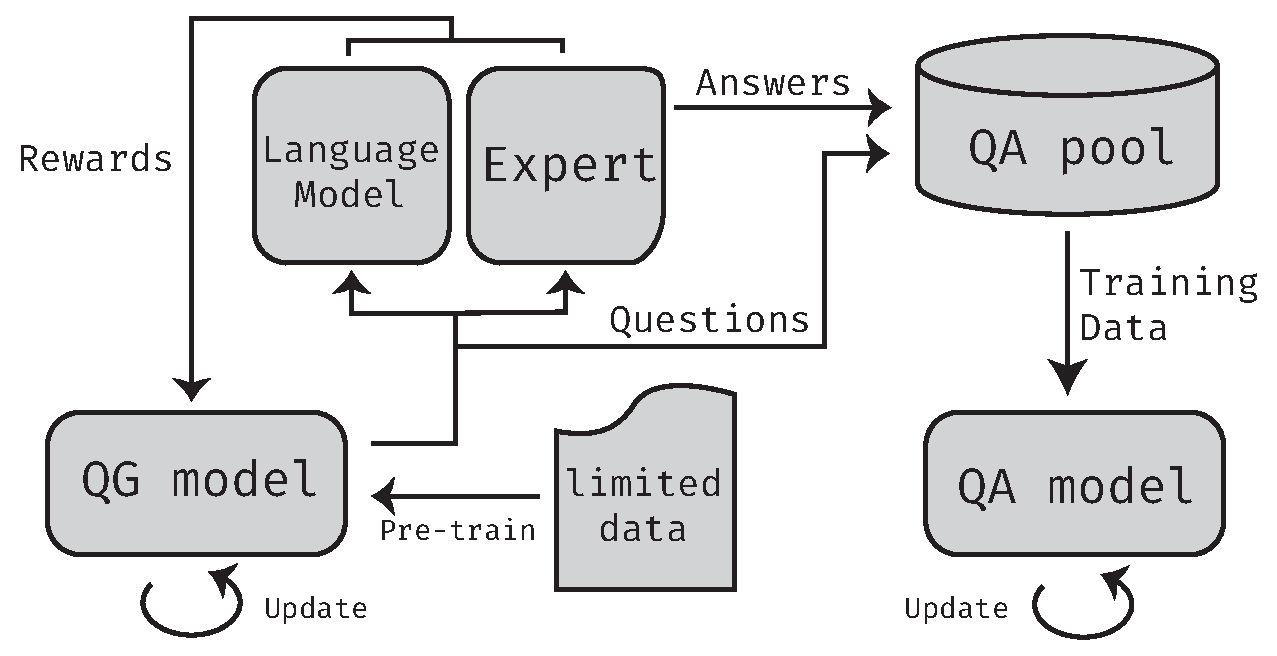
\includegraphics[width=0.9\linewidth]{fig/framework}
\caption{Framework}
\label{fig:framework}
\end{figure}

Figure \ref{fig:framework} shows our framework, which consists of an \emph{expert}, a \emph{language model}, and a \emph{learner}. The expert and the language model are prepared beforehand to give rewards to the generated questions during training. Specifically, the expert gives reward based on how confident it is to answer the given question while the language model gives reward based on the fluency. We emulate the expert using the recurrent entity network~\cite{hwsbl16:entnet}, which performs considerably well on the bAbI tasks, and use a simple RNN architecture~\cite{zsv14:language_model} for our language model.

The learner has two tasks: firstly, learning how to ask questions, and secondly, learning how to answer a variety of questions by exploiting the answers generated by the expert. The first task of learner is accomplished using a question generating model, which we call \emph{QG model}, and the second one is done using a question answering model, which we call \emph{QA model}. In the following text, we describe QA and QG model inside learner in more detail.

\subsection{Question generating model (QG model)}
We adapt Seq2seq model, which is first proposed in~\cite{cmgbsb14:seq2seq}, to the question generating task. In particular, the attention mechanism~\cite{bcb14:attention1, vkkpsh14:attention2, lpm15:Luong} is used. We will use $d_v$, $d_e$, and $d_h$ to represent vocabulary size, embedding size, and hidden size respectively in the following text.

The QG model outputs a \emph{question} $Q = (q_1, q_2, \ldots, q_m)$ given a \emph{document} $S = (s_1, s_2, \ldots, s_n)$. A \emph{document sentence vector}, $s_i \in \mathbb{R}^{d_e}$, is encoded from the $i$-th sentence in the document using positional encoding~\cite{sswf15:memn2n}.
%, which embeds a sentence not only with bag-of-words (BoW) representation but also with the information of the position of words.

A bidirectional LSTM~\cite{hs97:lstm} network is applied as an encoder, producing \emph{encoder hidden vectors} $h^e = (h^e_1, h^e_2, \ldots, h^e_n)$. Each of these encoder hidden vectors $h^e_i \in \mathbb{R}^{d_h}$ is an element-wise summation of $\overrightarrow{h^e_i}$ and $\overleftarrow{h^e_i}$.

The decoder of QG model is an LSTM with Luong attention mechanism (dot version)~\cite{lpm15:Luong} with the hidden state initialized as the last hidden state $h^e_n$ of the encoder. At each time step $t$, the decoder models a conditional distribution parametrized by $\theta$.
\begin{equation}
    \label{eq:decoder}
    \Pr\nolimits_{\theta}\left[y_t \mid y_{<t}, S\right]
\end{equation}
where $y_{<t}$ represents the outputs at all of the time steps earlier then $t$. On generating each $y_t$, they are sampled according to equation~\ref{eq:decoder}.

Given a \emph{decoder hidden state} $h^d_t$ at a certain time $t$ and the encoder hidden states $h^e$ of all time steps, the attention mechanism first computes an \emph{encoder context vector} $c_t$ that captures relevant encoder information to help predict the current word $y_t$ and then employs a simple concatenation layer which combines $h^d_t$ and $c_t$ to produce an \emph{attentional hidden state} $\tilde{h}^d_t$. Namely,
\begin{equation}
    \tilde{h}^d_t=W_c[c_t; h^d_t]
\end{equation}
where $W_c$ is a trainable matrix of size $2d_h \times d_v$. The attentional hidden state is then fed through the softmax layer directly to produce the predictive distribution.

There are many ways to compute the context vector $c_t$. We use the global attentional model~\cite{lpm15:Luong} with dot-version score function.

%An alignment vector $a_t$, whose size equals the number of time steps on the encoder side is computed as follows:

%\begin{equation}
    %a_t(s)=\frac{\exp({h^d_t}^\top h^e_s)}{\sum_{s'}\exp({h^d_t}^\top h^e_{s'})}
%\end{equation}

%Given that alignment vector as weights, the context vector $c_t$ is computed as the weighted average over all encoder hidden states.

We also use input-feeding approach~\cite{lpm15:Luong}, in which the input of decoder is the concatenation of previous attention vector $\tilde{h}^d_{t-1}$ and input word vector. Also, we feed the input word vector with ground truth in the training phase (also called \emph{teacher forcing}) while feed the word vector with previous generated word vector $y_{t-1}$ in the testing phase.

\subsection{Question answering model (QA model)}
The QA model predicts the answer given a document and a question. Although all answers are just one word long in bAbI and thus we can simplify the QA model to not use an RNN decoder, some of other QA tasks require the answer to be a sentence instead of a word. Hence, to make our model more general for other tasks, we still choose a seq2seq-like model, which in this case is just one step long though.

The document sentence vectors and encoder hidden vectors are generated according to the same architecture as that in QG model. However, all weights including embedding matrix etc. are not shared between QA and QG model. For question vectors, they are encoded by positional encoding~\cite{sswf15:memn2n} just like the way we encode the document sentence vectors.

To generate the answer, the LSTM with Luong attention mechanism (dot version) is used as the decoder. The only difference is the initial hidden state. Instead of initializing the decoder hidden state with the last encoder hidden vector, we initialize it with the question vector to make the prediction conditioned on the question.

\section{Training}
\label{sec:training}
\subsection{Supervised learning}
The QG model is trained initially to minimize the negative log-likelihood
\begin{equation}
    \mathcal{L}=-\sum_{t}\log \Pr\nolimits_\theta\left[y_t \mid y_{<t}, S\right]
\end{equation}

Similar is the QA model, which is trained with the loss function:
\begin{equation}
    \mathcal{L}=-\log \Pr\nolimits_\theta\left[y_1 \mid S\right]
\end{equation}
\subsection{Policy gradient}
\label{subsec:policy}
QG model only learns the one-to-one mapping from a document $S$ to a question $Q$ via supervised learning. In real world, however, there can be many questions which are all mapped from a document. Maximizing ground-truth likelihood does not teach the model how to distribute probability mass among examples other than the ground-truth. 
%Some of the generated questions may be valid and some of the generated questions may be completely incoherent. 
Therefore, we apply policy gradient method to fine-tune the QG model which has been pretrained on maximum likelihood. We use the REINFORCE algorithm~\cite{j92:reinforce} to maximize the model's expected reward. For each generated question $Q=(q_1,q_2,\ldots,q_m)$, we define the loss
\begin{equation}
\label{eq:rl_loss}
    \mathcal{L}_{\text{RL}}=-\mathbb{E}_{q\sim \pi(q \mid D)}\left[R(q)\right]
\end{equation}
where $\pi$ is the policy to be trained. 

REINFORCE approximates the expectation in the equation~\ref{eq:rl_loss} with independent samples from the policy distribution, yielding the policy gradient
\begin{equation}
    \mathcal{rL}_{\text{RL}}\approx\sum_{t}\mathcal{r}\log\pi(q_t \mid q_{<t}, S)\frac{R(q)-\mu_R}{\sigma_R}
\end{equation}
where $\mu_{R}$ and $\sigma_{R}$ are the running mean and standard deviation of the reward.
\subsection{Rewards}
%e ues four kinds of reward to measure questions' quality.
\subsubsection{Confidence of expert}
One obvious measurement of a question is the confidence of the expert, who answers it given the context document $S$. We feed questions generated from our QG model into the expert model, taking its output to compute rewards. In the beginning, we use cross entropy of answer probability as the reward function. 
%\begin{equation}
%    R_{\text{confidence}}=-\sum_{a\in A} p(a)\log(p(a))
%\end{equation}
%where A is probability distribution from expert, $A \in \mathbb{R}^{d_v}$. High probability of a certain answer leads to small cross entropy, which represents the expert's confidence of the answer.
However, we found there are 2 problems of this reward function. First, cross entropy is always close to 0, which means that the expert is very confident of its answer even though the question is irrelevant to the document. Another problem is that QG model tends to generate questions with bad grammar, such as repeated words, after applying policy gradient.

To solve the above problem, we use another function to represent the confidence of the expert:
\begin{equation}
    R_{\text{confidence}}=\frac{\text{max}(L)-\text{mean}(L)}{\text{std}(L)}
\end{equation}
where $L$ is the input of softmax layer, $A=\text{softmax}(L)$ and $L \in \mathbb{R}^{d_v}$. This reward deals with the first problem successfully, but the bad grammar problem remains. Therefore, we add other three rewards to eliminate it.

\subsubsection{Fluency}
Fluency is an important measurement of grammar. We use a language model to measure the fluency of generated questions. In particular, we use the perplexity assigned to $Q$ by the language model: 
\begin{equation}
    R_{\text{fluency}}=\left(\prod_{i=1}^{m}\Pr\nolimits_{\text{LM}}\left[q_i \mid q_{<i}\right]\right)^{\frac{-1}{m}}
    %R_{\text{fluency}}=\exp(\sum_{i=0}^{l}\frac{-\log\Pr_{LM}\left[q_i \mid q_{<i}\right]}{l})
\end{equation}
\subsubsection{Repeated words}

Let $\nu$ be the number of different words in $Q$ and $n_1,n_2\ldots,n_\nu$ be the numbers of each word appearing in $Q$.
We define
\begin{equation}
    R_{\text{repeat}}=\frac{\left(\sum_{i=0}^{\nu}n_i\right) - \nu}{m}
\end{equation}
Note that if all words in $Q$ are distinct, then $R_{\text{repeat}}=0$.

\subsubsection{Existence}

Because of the limited label data, QG model may generate questions irrelevant to D after pre-training. To eliminate this problem, we design a reward to check whether the question is relevant to D. Let $a=\text{argmax}(A)$.
\begin{equation}
    R_{\text{exist}} = \left\{
\begin{array}{ll}
0 & \text{, if }a \text{ is not in D}\\
1 & \text{, if }a \text{ is in D}\\
\end{array}
\right.
\end{equation}
Note that we assume if a question is relevant to D, then the answer of this question can be found in D.

Finally, total reward $R$ is the linear combination of the above rewards:
\begin{equation}
    R=R_{\text{confidence}}+(-0.1)R_{\text{fluency}}+(-4)R_{\text{repeat}}+R_{\text{exist}}
\end{equation}
\section{Experiments}
\label{sec:experiments}
%We use tensorflow\cite{tensorflow2015-whitepaper} to build our models.
Since the aim of our proposed framework is training a network with the ability to ask good questions which can be used to increase the total number of QA training pairs, we resort to the performance of the QA model within our learner to evaluate the quality of the questions generated by our QG model.

\subsection{Dataset}
Here we use the bAbI dataset as our question answering corpus. The bAbI dataset is a group of 20 synthetic question answering tasks provided by Weston et al.~\cite{wbcrmjm15:bAbI} designed for testing reasoning and text understanding. They have been utilized as a benchmark for many question answering models.

In previous works, proposed models are usually evaluated on each task of bAbI respectively. However, in order to reveal the ability of our framework, we blend the training sets of the first three tasks of bAbI into our evaluation set and design four training procedures for comparison.

\subsection{Evaluation Scheme}
The training procedures used in our evaluation scheme are described as follows. In order to simulate the situation of limited labeled data, where we can utilize our framework to generate extra QA training pairs, here we split the evaluation set into pre-train set and RL set with a certain labeling ratio. The data in pre-train set are preserved completely, while the data in RL set are discarded except the part of documents.
\begin{itemize}
%\subsubsection{Baseline}
    \item Baseline: 
         Before applying our framework for generating extra data, we first train our learner QA supervisedly with only the data in pre-train set. The result can be considered as the baseline of our proposed system.
%\subsubsection{RL}
    \item RL: 
        In this procedure, the proposed framework will be applied to generate extra data. The learner QG model will first be trained in supervised manner with pre-train set, followed by the process of policy gradient described in section~\ref{subsec:policy} performed with RL set. After we complete the two-stage training process, the trained QG model will be applied to the documents of RL set to generate new questions. Finally, the QA model of the learner, which the quality of generated questions can be evaluated with, will be trained with the new questions from RL set along with the data from pre-train set.
%\subsubsection{NonRL}
    \item NonRL: 
        We also design another method to train our learner QA model to show the effect of policy gradient on the quality of the generated questions. Instead of performing on QG model the two-stage training process, we directly apply the QG model to the RL set to generate new questions right after the pre-training on pre-train set, skipping the part of the policy gradient. The new generated QA pairs along with those in pre-train set will then be used to train the learner QA model.
%\subsubsection{Goal}
    \item Goal: 
        Finally, we train our learner QA model directly in supervised manner with all the labeled QA pairs in the evaluation set. The results can be seen as a presumed goal of the performance of our framework.%If our QG model is capable of generating questions that allow our QA model to achieve the results comparable to which are abtained by supervised training, the capability of our framework can then be well proven.
\end{itemize}

The four procedures will be performed with various labeling rate ranging from 10 percent to 90 percent to illustrate the impact of the difference on the amount of labeled data to the experimental results.
%\subsection{Implementation Details}
%In our experiments, the hyperparameters of the recurrent entity network used as our expert are set similar to that in \cite{hwsbl16:entnet}. While for the leaner QA and QG model, the embedding and hidden size are all set to 150. The hidden size of our language model is set to 650 in order to achieve the best performance on evaluating the fluency of our generated questions. All the model are trained via Adam\cite{DBLP:journals/corr/KingmaB14} with learning rate of 0.002, except for the policy gradient, whose learning rate is set to 0.0001. Regularization methods such as drop-out and batch normalization are also exploited in the training process.

\newcolumntype{Y}{>{\centering\arraybackslash}m{4.0em}}
\newcolumntype{X}{>{\centering\arraybackslash}m{3.0em}}
\begin{table}[t]
\small
\centering
\renewcommand{\arraystretch}{0.8}
\begin{tabular}{ XXXXYY }
\toprule
\multicolumn{1}{X}{\textbf{Label Ratio}} &
\multicolumn{1}{X}{\textbf{Baseline QA Acc}} &
\multicolumn{1}{X}{\textbf{RL QA Acc}} &
\multicolumn{1}{X}{\textbf{Goal QA Acc}} &
\multicolumn{1}{Y}{\textbf{Gain w.r.t Baseline}} &
\multicolumn{1}{Y}{\textbf{Gain w.r.t Goal}} \\
\midrule
0.1 & 0.612 & 0.811 & \multirow{9}{*}{0.910} & 32.6\% & -10.9\% \\
0.2 & 0.775 & 0.848 & & 9.49\% & -6.77\% \\
0.3 & 0.830 & 0.870 & & 4.78\% & -4.40\% \\
0.4 & 0.849 & 0.885 & & 4.19\% & -2.75\% \\
0.5 & 0.869 & 0.900 & & 3.57\% & -1.12\% \\
0.6 & 0.882 & 0.905 & & 2.56\% & -0.55\% \\
0.7 & 0.883 & 0.910 & & 3.02\% & 0.00\% \\
0.8 & 0.912 & 0.915 & & 0.33\% & 0.55\% \\
0.9 & 0.913 & 0.917 & & 0.48\% & 0.81\% \\
\bottomrule
\end{tabular}
\caption{Accuracy gain by means of QG framework}
\label{table:gain}
\end{table}

\subsection{Experimental Results}
In order to demonstrate the capability of our question generating framework, we first compare the results of the ``Baseline'' and ``RL'' procedures.% under different circumstances of limited data, we train the learner QA model following the four procedures mentioned earlier with various labeling ratio ranging from 10 percent to 90 percent.
The outcome accuracy on the testing set of the learner QA model trained by these two procedures are shown in Table~\ref{table:gain}. The relative differences of the accuracy between ``Baseline'' and ``RL'' procedures are also calculated. The performance of the QA model is improved considerably with the help of extra questions generated by the QG model, especially under the condition of low labeling ratio, which proves the quality of questions generated by our framework.

\begin{figure}[t]
    \centering
    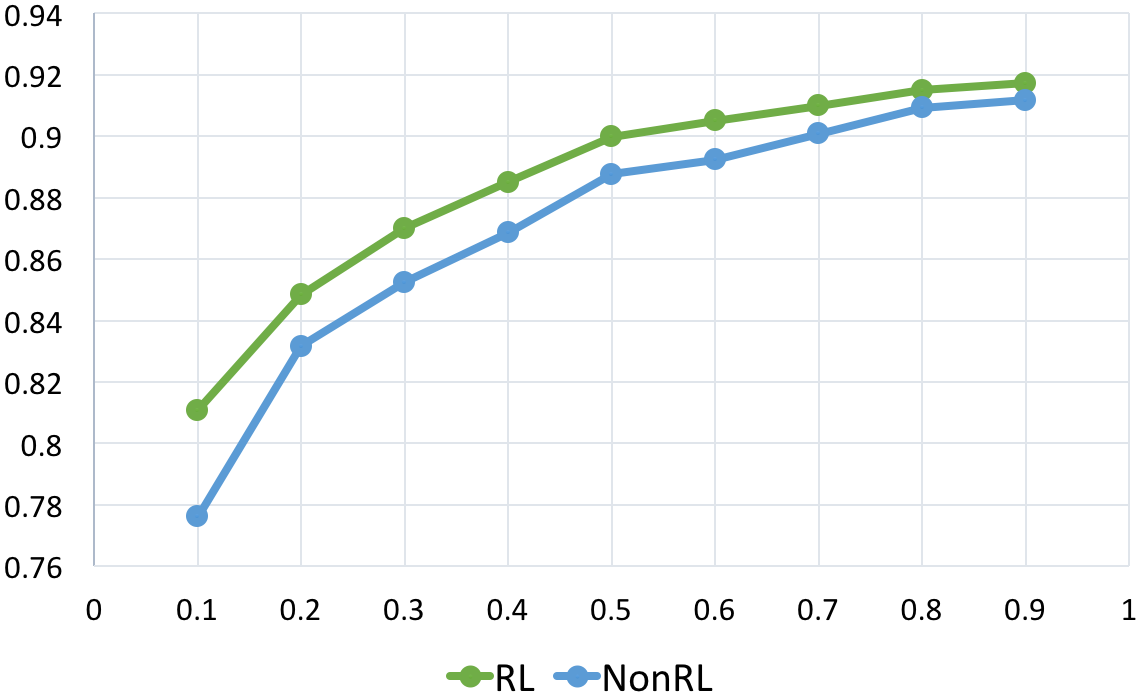
\includegraphics[width=0.95\linewidth]{fig/QA_acc.png}
    \caption{Accuracy of QA trainied by ``NonR’’ and ``RL’’ procedure under various labeling ratio}
    \label{fig:QA_acc}
\end{figure}

Furthermore, in regards to the comparison between ``RL'' and ``Goal'', the accuracy gains under the labeling ratio over 60 percent are all greater than -0.6 percent, as shown in Table~\ref{table:gain}. This results indicates that with the questions generating framework, our learner QA can achieve the comparable performance with the model accessible to the complete data even though only the 60 percent of the data are provided.

On the other hand, the final accuracy of the QA model trained by ``NonRL'' procedures are shown in figure~\ref{fig:QA_acc} along with the result of ``RL'' procedure. From the results, we can see that the accuracy curve of ``RL'' are always above that of ``NonRL'', which suggests that the policy gradient process are beneficial for generating good-quality questions. Besides, by comparing between the different labeling ratio, the results show that the effectiveness of the policy gradient is increasing as the ratio declines, which meets our expectation since what we want is exactly a framework that is useful under the condition of limited data. While in the situation of high labeling ratio, the accuracy gain is insignificant because the amount of labeling data is sufficient for the QG model to fit by supervised training.

%& Loss & Acc & Loss & Acc & Loss & Acc \\
%\midrule
 %0.1 & \multirow{9}{*}{0.440} & \multirow{9}{*}{0.910} & 1.356 & 0.776 & 1.012 & 0.811 & -10.9\% & 4.47\% \\
 %0.2 & & & 1.021 & 0.832 & 0.839 & 0.848 & -6.77\% & 2.03\% \\
 %0.3 & & & 0.906 & 0.853 & 0.765 & 0.870 & -4.40\% & 2.05\% \\
 %0.4 & & & 0.826 & 0.869 & 0.668 & 0.885 & -2.75\% & 1.89\% \\
 %0.5 & & & 0.711 & 0.888 & 0.581 & 0.900 & -1.12\% & 1.37\% \\
 %0.6 & & & 0.719 & 0.892 & 0.563 & 0.905 & -0.55\% & 1.42\% \\
 %0.7 & & & 0.647 & 0.901 & 0.542 & 0.910 & 0.00\% & 1.02\% \\
 %0.8 & & & 0.605 & 0.909 & 0.527 & 0.915 & 0.55\% & 0.64\% \\
 %0.9 & & & 0.601 & 0.912 & 0.513 & 0.917 & 0.81\% & 0.62\% \\
%0.1 & 1.36 & 0.70 \\
%0.2 & 1.27 & 0.72 \\
%0.3 & 1.14 & 0.76 \\
%0.4 & 1.15 & 0.76 \\
%0.5 & 1.17 & 0.75 \\
%0.6 & 1.12 & 0.75 \\
%0.7 & 1.16 & 0.76 \\
%0.8 & 1.20 & 0.74 \\
%0.9 & 1.13 & 0.75 \\
%\end{tabular}
%\caption{Task 2 nonRL}
%\end{minipage}
%\hfill
%\begin{minipage}[b]{0.48\linewidth}
%\centering
%\begin{tabular}{ l | l | l }
%ratio & loss & acc \\
%\hline
%0.1 & 1.18 & 0.75 \\
%0.2 & 1.07 & 0.77 \\
%0.3 & 1.12 & 0.75 \\
%0.4 & 1.16 & 0.74 \\
%0.5 & 1.13 & 0.76 \\
%0.6 & 1.14 & 0.75 \\
% 0.7 & 1.04 & 0.77 \\
%0.8 & 1.06 & 0.77 \\
%0.9 & 1.07 & 0.77 \\
%\end{tabular}
%\caption{Task 2 RL}
%\end{minipage}
%\end{table}
\section{Conclusion}
\label{sec:conclusion}
In this paper, we design a novel framework including an expert and a learner to address the problem of limited training data, which is an important issue in the field of question answering. The experimental results show that in the circumstance of limited training QA pairs, our proposed system can not only generate high-quality questions which improve the accuracy of a QA model, a QA model whose performance is comparable with those trained by unlimited data can also be achieved with the help of reinforcement learning.

%\pagebreak

\bibliographystyle{IEEEbib}
\bibliography{refs}

\end{document}
